In this section, we evaluate the performance of the proposed techniques. All the
experiments are conducted on a GNU/Linux machine equipped with 16 processors
Intel Xeon E5520 2.27~GHz and 24~GB of RAM.

Heterogeneous platforms and applications are generated by the \abbr{TGFF} tool
\cite{dick1998}. For each considered configuration/problem, the tool generates
(i) a directed acyclic graph representing tasks along with their data
dependencies and (ii) a number of tables representing processing elements. Each
table assigns two numbers to each task: a best-case execution time and a power
consumption. The two numbers characterize the task when it is being executed on
the processing element that the table corresponds to. The best-case execution
time is chosen uniformly between 1 and 50~ms, and it is used for assigning a
probability distribution to the execution time of the task, which will be
discussed shortly. The power consumption is chosen uniformly between 10 and
50~W, and it is assumed to remain fixed thereafter. The floorplans of the
platforms are constructed as regular grids wherein each processing element
occupies $4 \times 4~\text{mm}^2$ on the die.

\begin{figure}[t]
  \centering
  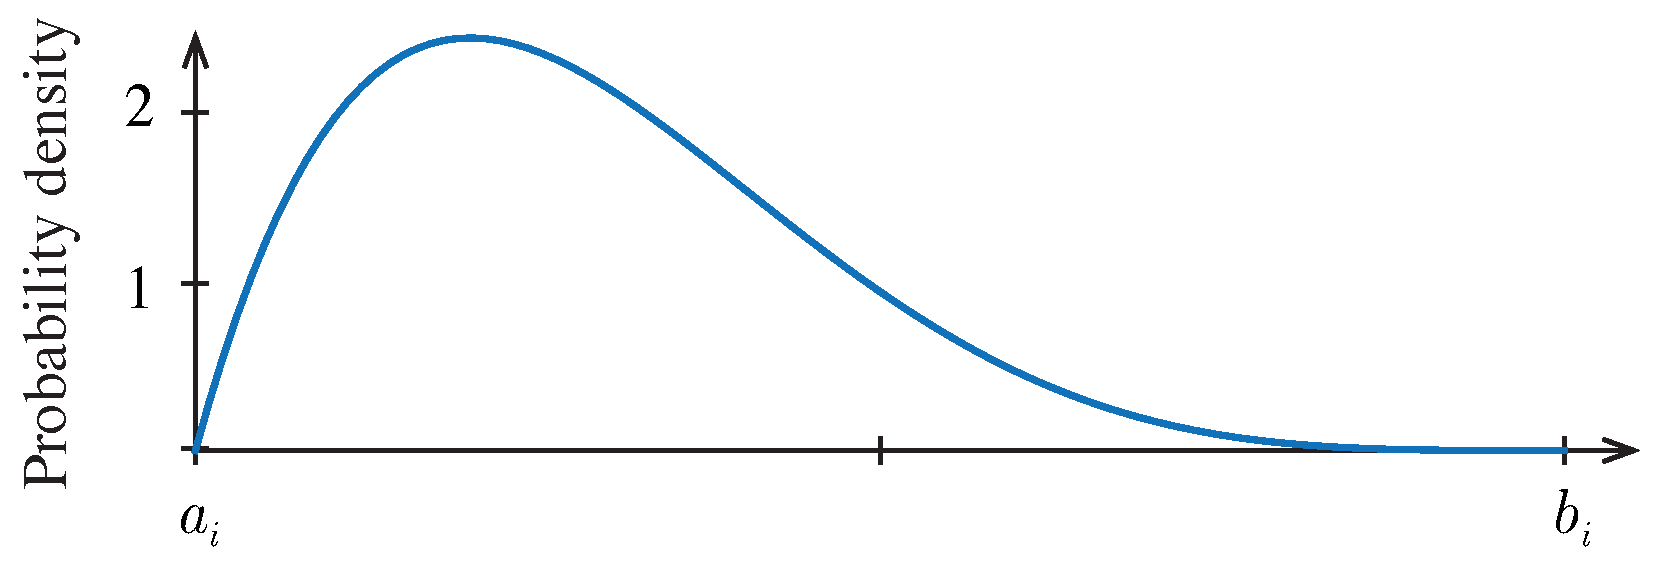
\includegraphics[width=1.0\columnwidth]{include/assets/beta.pdf}
  \caption{The probability density of the beta distribution $\text{Beta}(2, 5, a_i, b_i)$.}
  \flab{beta}
\end{figure}

For illustration purposes, the uncertain parameters are assumed to be the
execution times of the tasks; in other words, $\vu = \vb$ and $\nu = \nt$.
Without loss of generality, the distribution of $\u_i$ or, equivalently, $\b_i$
is assumed to be a four-parametric beta distribution $\text{Beta}(\alpha_i,
\beta_i, a_i, b_i)$ where $\alpha_i$ and $\beta_i$ are the shape parameters, and
$a_i$ and $b_i$ are the endpoints of the support. The parameters $\alpha_i$ and
$\beta_i$ are set to 2 and 5, respectively, for all tasks; the shape of such
distributions is depicted in \fref{beta}. The left endpoint $a_i$ is set to the
best-case execution time of the task as generated by the \abbr{TGFF} tool, and
the right endpoint $b_i$ is set to $1.2 \times a_i$.

\subsection{Application Timing}
The quantity of interest $\g$ considered in this subsection is the end-to-end
delay given in \eref{end-to-end-delay}, which is a scalar.

\subsection{Power Consumption}
Let the quantity of interest $\g$ be the total energy given in
\eref{total-energy}, which is a scalar.

\subsection{Heat Dissipation}
In this subsection, the quantity of interest $\g$ is the temperature profile
$\mQ$ of the system calculated using \eref{thermal-system}. The profile is an
$\np \times \ns$ matrix, and, therefore, $\g$ is $\np \ns$-dimensional.

The granularity of power and temperature profiles, discussed in
\sref{power-consumption} and \sref{heat-dissipation}, is set to $10^{-5}$~s; in
practice, this sampling interval should be set to a value that is reasonable for
the problem at hand. Thermal RC circuits---which are essentially pairs of a
thermal capacitance matrix $\mC$ and a thermal conductance $\mG$ matrix in
\eref{thermal-system}---are constructed using the HotSpot thermal model
\cite{skadron2004}.
